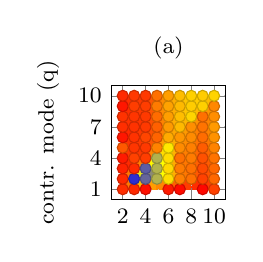
\begin{tikzpicture}
\begin{axis}
[
width=0.25\textwidth,
height=0.25\textwidth,
style={font=\footnotesize},
grid=major,
grid style={dotted},
align=center,
%xlabel={tensor order},
ylabel={contr. mode (q)},
title={{(a)}}, %  ompfor<slice>, asymmetric, row-major
scaled ticks=false,
zlabel={GFlops/core},
view={0}{90}, 
%view={-45}{45}, 
ytick={1,4,7,10},
xtick={2,4,6,8,10},
xmin=1, xmax=11,
ymin=0, ymax=11,
try min ticks=8,
zmin=0, zmax=50,
point meta min=0, point meta max=50,
colormap/hot, 
samples=50,
]
\addplot3[contour filled={number=100},scatter,shader=flat,samples=50]
coordinates{

(2.000,1.000,43.896) (2.000,2.000,44.316) (2.000,3.000,45.340) (2.000,4.000,46.159) (2.000,5.000,38.284) (2.000,6.000,46.700) (2.000,7.000,43.782) (2.000,8.000,43.238) (2.000,9.000,46.586) (2.000,10.000,44.445) 

(3.000,1.000,44.157) (3.000,2.000,3.488) (3.000,3.000,44.009) (3.000,4.000,41.443) (3.000,5.000,42.540) (3.000,6.000,43.421) (3.000,7.000,43.343) (3.000,8.000,42.638) (3.000,9.000,41.938) (3.000,10.000,42.175) 

(4.000,1.000,47.610) (4.000,2.000,6.548) (4.000,3.000,6.497) (4.000,4.000,41.914) (4.000,5.000,42.480) (4.000,6.000,40.513) (4.000,7.000,42.150) (4.000,8.000,42.362) (4.000,9.000,41.508) (4.000,10.000,42.485) 

(5.000,1.000,51.579) (5.000,2.000,11.839) (5.000,3.000,11.713) (5.000,4.000,11.721) (5.000,5.000,32.597) (5.000,6.000,36.602) (5.000,7.000,37.323) (5.000,8.000,35.667) (5.000,9.000,33.893) (5.000,10.000,35.328) 

(6.000,1.000,46.209) (6.000,2.000,21.375) (6.000,3.000,21.542) (6.000,4.000,21.382) (6.000,5.000,19.695) (6.000,6.000,27.921) (6.000,7.000,29.645) (6.000,8.000,29.213) (6.000,9.000,28.661) (6.000,10.000,29.405) 

(7.000,1.000,48.068) (7.000,2.000,33.377) (7.000,3.000,33.695) (7.000,4.000,35.053) (7.000,5.000,31.593) (7.000,6.000,30.136) (7.000,7.000,25.612) (7.000,8.000,25.054) (7.000,9.000,25.955) (7.000,10.000,25.248) 

(8.000,1.000,50.865) (8.000,2.000,35.412) (8.000,3.000,35.133) (8.000,4.000,33.799) (8.000,5.000,33.342) (8.000,6.000,31.890) (8.000,7.000,31.426) (8.000,8.000,22.371) (8.000,9.000,23.403) (8.000,10.000,22.843) 

(9.000,1.000,48.543) (9.000,2.000,41.355) (9.000,3.000,40.444) (9.000,4.000,39.428) (9.000,5.000,37.619) (9.000,6.000,35.552) (9.000,7.000,34.559) (9.000,8.000,35.278) (9.000,9.000,22.785) (9.000,10.000,23.178) 

(10.000,1.000,41.434) (10.000,2.000,36.469) (10.000,3.000,36.005) (10.000,4.000,34.970) (10.000,5.000,32.842) (10.000,6.000,30.760) (10.000,7.000,29.786) (10.000,8.000,31.179) (10.000,9.000,32.441) (10.000,10.000,22.265) 

};
\end{axis}
\end{tikzpicture}
\hfill
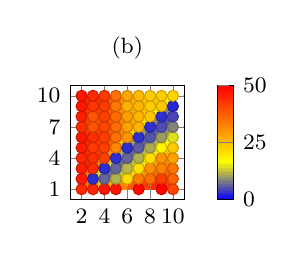
\begin{tikzpicture}
\begin{axis}
[
width=0.25\textwidth,
height=0.25\textwidth,
style={font=\footnotesize},
grid=major,
grid style={dotted},
align=center,
%xlabel={tensor order},
%ylabel={contr. mode (q)},
title={{(b)}}, %  ompfor<subtensor>, asymmetric, mkl
scaled ticks=false,
zlabel={GFlops},
view={0}{90}, 
ytick={1,4,7,10},
xtick={2,4,6,8,10},
xmin=1, xmax=11,
ymin=0, ymax=11,
try min ticks=8,
zmin=0, zmax=50,
point meta min=0, point meta max=50,
colormap/hot, 
samples=50,
colorbar sampled,
colorbar/width=0.2cm,
colorbar style={
	point meta min=0, point meta max=50,
	samples=50,
	font=\footnotesize,
	ytick={0,25,50},
	yticklabels={0,25,50},
	%title={\scriptsize Gflops},
	%ylabel={\scriptsize Gflops},
}
]
\addplot3[contour filled={number=100},scatter,shader=flat,samples=50]
coordinates{

(2.000,1.000,44.459) (2.000,2.000,46.351) (2.000,3.000,45.510) (2.000,4.000,44.636) (2.000,5.000,46.447) (2.000,6.000,46.641) (2.000,7.000,43.856) (2.000,8.000,45.859) (2.000,9.000,46.509) (2.000,10.000,46.686) 

(3.000,1.000,44.727) (3.000,2.000,3.490) (3.000,3.000,44.197) (3.000,4.000,43.861) (3.000,5.000,42.244) (3.000,6.000,43.848) (3.000,7.000,38.887) (3.000,8.000,38.650) (3.000,9.000,42.539) (3.000,10.000,44.223) 

(4.000,1.000,46.771) (4.000,2.000,6.537) (4.000,3.000,3.497) (4.000,4.000,41.114) (4.000,5.000,41.946) (4.000,6.000,41.889) (4.000,7.000,40.607) (4.000,8.000,41.455) (4.000,9.000,42.025) (4.000,10.000,41.998) 

(5.000,1.000,46.889) (5.000,2.000,11.964) (5.000,3.000,6.581) (5.000,4.000,3.465) (5.000,5.000,32.495) (5.000,6.000,35.170) (5.000,7.000,35.654) (5.000,8.000,35.862) (5.000,9.000,34.450) (5.000,10.000,35.248) 

(6.000,1.000,50.072) (6.000,2.000,21.383) (6.000,3.000,12.015) (6.000,4.000,6.500) (6.000,5.000,3.352) (6.000,6.000,30.066) (6.000,7.000,28.556) (6.000,8.000,29.463) (6.000,9.000,26.748) (6.000,10.000,28.155) 

(7.000,1.000,48.039) (7.000,2.000,33.621) (7.000,3.000,20.592) (7.000,4.000,11.558) (7.000,5.000,6.048) (7.000,6.000,3.278) (7.000,7.000,26.467) (7.000,8.000,26.394) (7.000,9.000,26.159) (7.000,10.000,25.519) 

(8.000,1.000,50.776) (8.000,2.000,35.546) (8.000,3.000,31.023) (8.000,4.000,20.828) (8.000,5.000,11.065) (8.000,6.000,5.837) (8.000,7.000,3.102) (8.000,8.000,24.096) (8.000,9.000,23.135) (8.000,10.000,23.270) 

(9.000,1.000,49.071) (9.000,2.000,41.747) (9.000,3.000,33.411) (9.000,4.000,30.777) (9.000,5.000,18.497) (9.000,6.000,10.262) (9.000,7.000,5.464) (9.000,8.000,3.133) (9.000,9.000,23.542) (9.000,10.000,23.357) 

(10.000,1.000,40.520) (10.000,2.000,37.272) (10.000,3.000,34.697) (10.000,4.000,28.652) (10.000,5.000,23.911) (10.000,6.000,14.900) (10.000,7.000,8.805) (10.000,8.000,4.918) (10.000,9.000,2.844) (10.000,10.000,22.469) 

};
\end{axis}
\end{tikzpicture}
\hfill
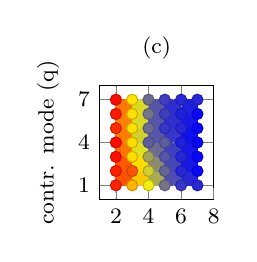
\begin{tikzpicture}
\begin{axis}
[
width=0.25\textwidth,
height=0.25\textwidth,
style={font=\footnotesize},
grid=major,
grid style={dotted},
align=center,
%xlabel={tensor order},
ylabel={contr. mode (q)},
title={{(c)}}, %  ompfor<slice>, symmetric, row-major
scaled ticks=false,
zlabel={GFlops},
view={0}{90}, 
ytick={1,4,7,10},
xtick={2,4,6,8},
xmin=1, xmax=8,
ymin=0, ymax=8,
try min ticks=8,
zmin=0, zmax=55,
point meta min=0, point meta max=55,
colormap/hot, 
samples=50,
]
\addplot3[contour filled={number=100},scatter,shader=flat,samples=50]
coordinates{

(2.000,1.000,49.884) (2.000,2.000,50.237) (2.000,3.000,52.259) (2.000,4.000,53.112) (2.000,5.000,48.642) (2.000,6.000,51.140) (2.000,7.000,53.264) 

(3.000,1.000,29.064) (3.000,2.000,42.832) (3.000,3.000,23.356) (3.000,4.000,23.347) (3.000,5.000,22.695) (3.000,6.000,22.978) (3.000,7.000,22.478) 

(4.000,1.000,17.083) (4.000,2.000,15.195) (4.000,3.000,12.081) (4.000,4.000,6.961) (4.000,5.000,8.128) (4.000,6.000,8.480) (4.000,7.000,8.210) 

(5.000,1.000,8.642) (5.000,2.000,7.699) (5.000,3.000,6.147) (5.000,4.000,6.635) (5.000,5.000,4.357) (5.000,6.000,4.476) (5.000,7.000,4.664) 

(6.000,1.000,4.335) (6.000,2.000,3.270) (6.000,3.000,2.956) (6.000,4.000,2.500) (6.000,5.000,2.807) (6.000,6.000,2.631) (6.000,7.000,2.772) 

(7.000,1.000,3.151) (7.000,2.000,0.567) (7.000,3.000,0.638) (7.000,4.000,0.650) (7.000,5.000,0.632) (7.000,6.000,0.649) (7.000,7.000,2.781) 


};
\end{axis}
\end{tikzpicture}
\hfill
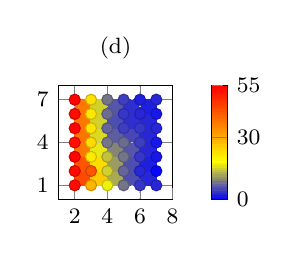
\begin{tikzpicture}
\begin{axis}
[
width=0.25\textwidth,
height=0.25\textwidth,
style={font=\footnotesize},
grid=major,
grid style={dotted},
align=center,
%xlabel={tensor order},
%ylabel={contr. mode (q)},
title={{(d)}}, %  ompfor<subtensor>, symmetric, row-major
scaled ticks=false,
zlabel={GFlops},
view={0}{90}, 
%view={-45}{45}, 
ytick={1,4,7,10},
xtick={2,4,6,8},
xmin=1, xmax=8,
ymin=0, ymax=8,
try min ticks=8,
zmin=0, zmax=55,
point meta min=0, point meta max=55,
colormap/hot, 
samples=50,
colorbar sampled,
colorbar/width=0.2cm,
colorbar style={
	point meta min=0, point meta max=55,
	samples=50,
	font=\footnotesize,
	ytick={0,30,55},
	yticklabels={0,30,55},
	%title={\scriptsize Gflops},
	%ylabel={\scriptsize Gflops},
}
]
\addplot3[contour filled={number=100},scatter,shader=flat,samples=50]
coordinates{

(2.000,1.000,52.847) (2.000,2.000,53.105) (2.000,3.000,54.140) (2.000,4.000,52.620) (2.000,5.000,53.976) (2.000,6.000,53.003) (2.000,7.000,53.953) 

(3.000,1.000,28.660) (3.000,2.000,42.680) (3.000,3.000,21.118) (3.000,4.000,23.419) (3.000,5.000,22.416) (3.000,6.000,21.925) (3.000,7.000,22.886) 

(4.000,1.000,17.375) (4.000,2.000,15.257) (4.000,3.000,13.767) (4.000,4.000,8.621) (4.000,5.000,7.667) (4.000,6.000,7.963) (4.000,7.000,8.423) 

(5.000,1.000,8.648) (5.000,2.000,7.667) (5.000,3.000,8.572) (5.000,4.000,7.742) (5.000,5.000,4.437) (5.000,6.000,4.127) (5.000,7.000,4.642) 

(6.000,1.000,4.295) (6.000,2.000,3.270) (6.000,3.000,4.016) (6.000,4.000,4.522) (6.000,5.000,3.888) (6.000,6.000,2.759) (6.000,7.000,2.713) 

(7.000,1.000,3.143) (7.000,2.000,0.571) (7.000,3.000,1.910) (7.000,4.000,1.785) (7.000,5.000,2.751) (7.000,6.000,1.807) (7.000,7.000,3.058) 


};
\end{axis}
\end{tikzpicture}